\documentclass{article}

\usepackage[utf8]{inputenc}
\usepackage[T1]{fontenc}
\usepackage{mathptmx}
\usepackage{geometry}
\usepackage{mathtools}
\usepackage{hyperref}

\usepackage[english]{babel}
 \usepackage{minted}

\geometry{
 a4paper,
 left=25mm,
 right=15mm,
 top=25mm,
 bottom=15mm, 
}
 
\renewcommand{\baselinestretch}{1.0}
\makeatletter
\renewcommand\normalsize{\@setfontsize\normalsize{11}{15}}
\renewcommand\large{\@setfontsize\large{13}{15}}
\makeatother
\pagenumbering{gobble}

% ===============================================================

\begin{document}

\title{Internal Combustion Engine Parametric Modelling}
\author{Achmadi - 2416201010}
\date{\vspace{-5ex}}

\maketitle


In this summary, we will explain how to get mathematical equation as model for an Internal Combustion Engine.
All file can be found at:\\
\url{https://github.com/mekatronik-achmadi/tugas_kuliah/tree/master/Identification_System}

\section{Engine Data}

In order to build parametric equation model, we must have some input-output data from system.
Based on this data then we can build the model.
We choose data from Sapu Angin engine test.
The Data field we get are:
\begin{itemize}
	\item Throttle Position as ADC bit feed
	\item Combustion Start Degree
	\item Mass Fuel Flow rate
	\item Rotation Per Minutes
	\item Torque
	\item Air to Fuel Ratio
\end{itemize} 

In this work, the last two data are not used due to process simplification.
Total amount data row is 150.\\
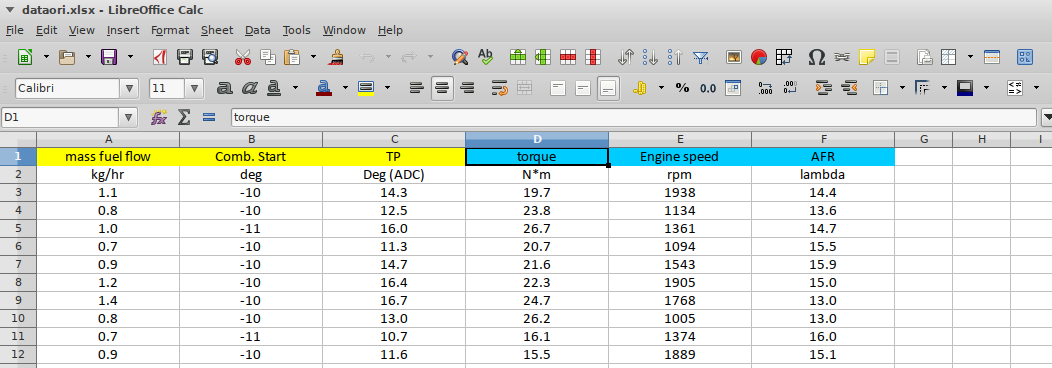
\includegraphics[width=500pt]{data}\\

\section{Model Equation}
As conventional known that engine process or other mechanical process, take only instantaneous response.
So using only one step back response should be sufficient.
The mathematical model proposed are:\\

\hspace{10pt} $y_n = ay_{n-1} + bu_n + cu_{n-1} + dv_n + ev_{n-1} + fw_n + gw_{n-1}$\\

and:

\noindent$y =$ rotation per minute\\
$u =$ throttle position\\
$v =$ combustion start degree\\
$w =$ mass fuel flow rate

\section{Least Square Method}

Least Square Method defined by following step:

\subsection{Build Matrix}
From defined equation we build following matrix:
\[
\begin{bmatrix}
    y \\
\end{bmatrix}
=
\begin{bmatrix}
	y_{n-1} & u_n & u_{n-1} & v_n & v_{n-1} & w_n & w_{n-1} \\
\end{bmatrix}
\begin{bmatrix}
    a \\
    b \\
    c \\
    d \\
    e \\
    f \\
    g \\
\end{bmatrix}
\]

and we rewrite as $Y = \phi^T * \theta$

\subsection{Get Coeffisient Matrix ($\theta$)}
Matrix H on Least Square define as:\\

$\theta = (\phi^T\phi)^{-1}\phi^TY $ 

\subsection{Calculate using Software}
Last step is implement this method on software for much easier calculation process.
We use Python since it's free and open-source.
Python platfrom we used mainly is NumPy with help Scipy and Matplotlib.
We divide data into two groups, first 125 for build equation and the reat 25 data for validation.
Here's the code:\\
\inputminted{python}{least_square.py}

% ===============================================================
\newpage

\section{Result}
Here the plot to compare measured and estimated for last 25 data:\\
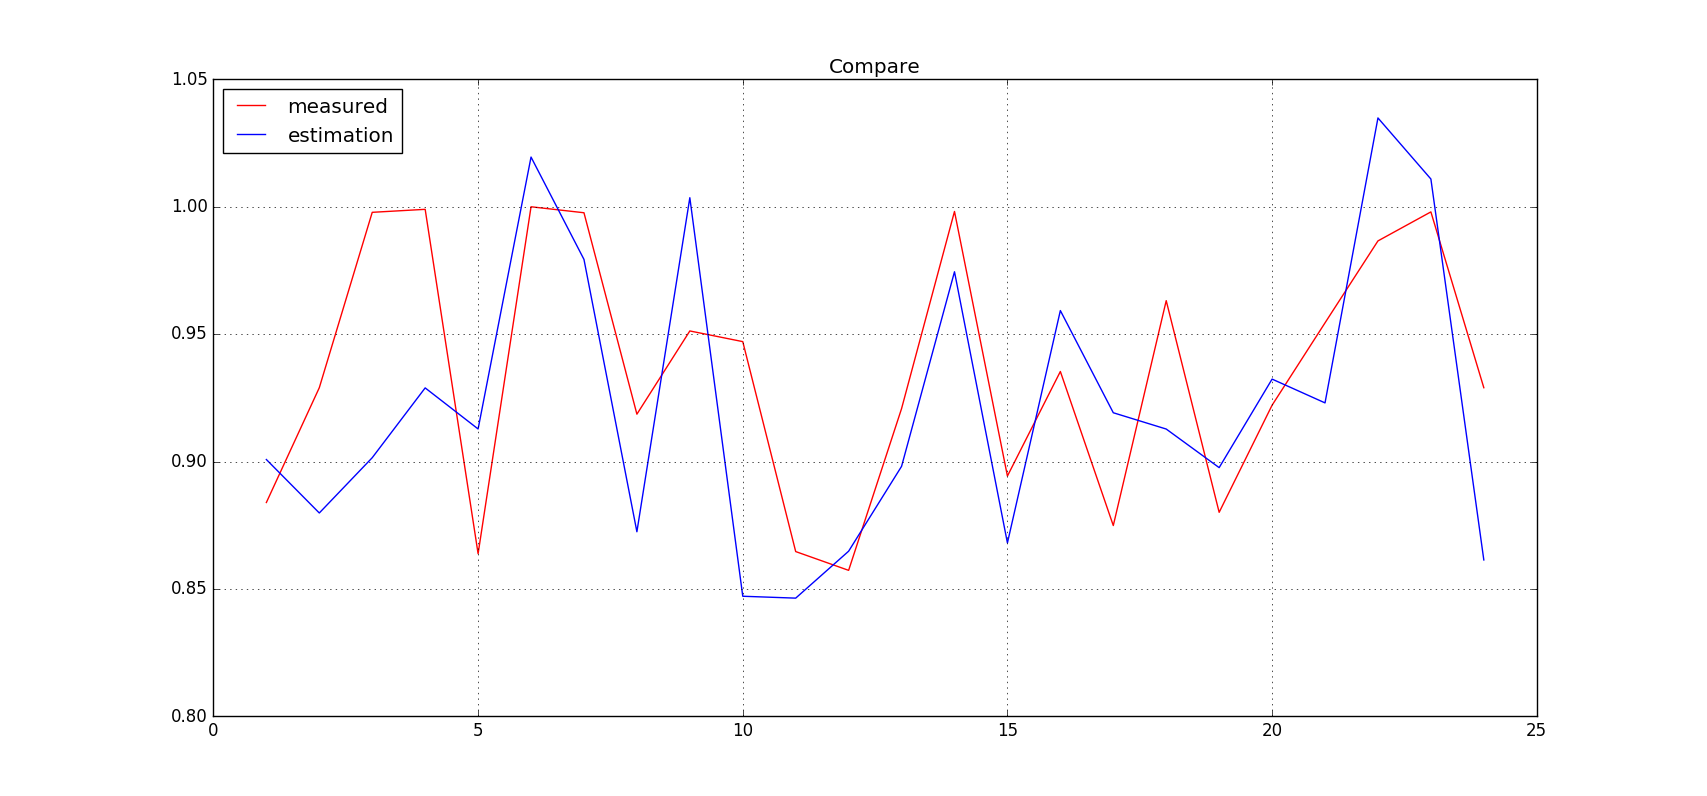
\includegraphics[width=500pt]{komparasi}\\

\end{document}
